\subsection{Лемма Пуанкаре для когомологий де Рама}

 	\begin{remark}
 		В этом параграфе мы не пользуемся обозначением $\wedge$ для внешнего произведения. А может быть, стоило. 
 	\end{remark}

 		Рассмотрим диаграммы: 

 		\begin{center}
 			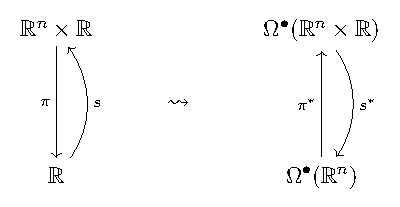
\includegraphics{lectures/7/pictures/cd_12.pdf}
 		\end{center}

 		где $\pi$~--- проекция на первые $n$ координат (т.е. $\pi(x, t) = x$), а $s$~--- сечение, т.е. $s(x) = (x, 0)$. Покажем, что отображения $\pi \circ s$ и $s \circ \pi$ индуцируют изоморфизм на когомологиях. 

 		Во-первых, по очевидным причинам $\pi \circ s = \id$, откуда $s^* \circ \pi^* = \id$ (т.е. отображение тождественно уже на уровне форм, а значит, индуцирует изоморфизм на когомологиях). Но вот $s \circ \pi(x, t) = (x, 0)$ и отображение $\pi^* \circ s^*$ уже не тождественно на уровне форм (например, оно переводит $f(x, t)$ в $f(x, 0)$). Но изоморфизм в когомологиях оно всё-таки индуцирует. Чтоб доказать это, мы покажем, что $\pi^* \circ s^*$ цепно-гомотопно тождественному:
 		\[
 		 	\id - \pi^* \circ s^* = \pm (\mathrm{d}K \pm K\mathrm{d}).
 		 \] 

 		 Как мы помним, цепно-гомотопные отображения индуцируют одинаковые отображения в когомологиях, так что этого достаточно. 

 		 Заметим, что любая форма на $\R^n \times \R$ представляется в виде линейной комбинации форм одного из двух видов: 
 		 \begin{enumerate}
 		 	\item $(\pi^* \varphi) f(x, t)$
 		 	\item $(\pi^*\varphi) f(x, t) \mathrm{d}t$,
 		 \end{enumerate}
 		 так как там либо есть $\mathrm{d}t$, либо нет. 

 		 Посмотрим сначала, как $s^*$ действует на формы. Рассмотрим форму $f(x, t) \mathrm{d}x_{I} \wedge \mathrm{d}t$. Тогда, так как $s^*(\mathrm{d}t) = 0$, $s^*(f(x, t) \mathrm{d}x_{I} \wedge \mathrm{d}t) = 0$. Если же сверху у нас форма $f(x, t) \mathrm{d}x_I$, то $s^*(f(x, t) \mathrm{d}x_I) = f(x, 0) \mathrm{d}x_I$. 

 		 Теперь определим $K\colon \Omega^q(\R^n \times \R) \to \Omega^{q - 1}(\R^n \times \R)$ следующим образом: 
 		 \[
 		 	K\lr*{ (\pi^* \varphi) f(x, t) } = 0, \quad K\lr*{ (\pi^*\varphi) f(x, t) \mathrm{d}t } = (\pi^* \varphi) \int\limits_{0}^{t} f(s, t) \mathrm{d}s.
 		 \]

 		 Проверим, что $K$ действительно является оператором цепной гомотопии. Само собой, это достаточно проверять отдельно на функциях двух типов: 

 		 \begin{itemize}
 		 	\item Пусть $\omega = (\pi^* \varphi) f(x, t)$, $\deg{\omega} = q$. Тогда 
 		 	\[
 		 		(\id - \pi^* \circ s^*) \omega = (\pi^* \varphi) f(x, t) - (\pi^* \varphi) f(x, 0).
 		 	\]
 		 	В то же время, так как $K$ ноль на формах первого типа, 
 		 	\[
 		 		(\mathrm{d}K - K\mathrm{d})\omega = -K\mathrm{d}\omega.
 		 	\]
 		 	\[
 		 		\mathrm{d}\lr*{ (\pi^*\varphi)f(x, t) } = \mathrm{d}\pi^*\varphi \cdot f(x, t) + (-1)^q \pi^* \varphi \cdot \lr*{\sum_{j = 1}^n \frac{\partial f}{\partial x_j}(x, t) \mathrm{d}x_j + \frac{\partial f(x, t)}{\partial t} \mathrm{d}t}. 
 		 	\]
 		 	\[
 		 		K\lr*{ \mathrm{d}\pi^*\varphi \cdot f(x, t) + (-1)^q \pi^* \varphi \cdot \lr*{\sum_{j = 1}^n \frac{\partial f}{\partial x_j}(x, t) \mathrm{d}x_j + \frac{\partial f(x, t)}{\partial t} \mathrm{d}t} }.
 		 	\]
 		 	теперь заметим, что в первых двух слагаемых $\mathrm{d}t$ нет, поэтому $K$ их занулит. На остальное он подействует вот так: 
 		 	\[
 		 		-K\lr*{ (-1)^q \pi^* \varphi \cdot \frac{\partial f(x, t)}{\partial t} \mathrm{d}t } = (-1)^{q - 1} \pi^* \varphi \int\limits_{0}^t \frac{\partial f(x, t)}{\partial t} \mathrm{d}t = (-1)^{q - 1} \pi^* \varphi \lr*{ f(x, t) - f(x, 0) }. 
 		 	\]
 		 	Таким образом, на формах первого типа мы получили 
 		 	\[
 		 		\id - \pi^* \circ s^* = (-1)^{q - 1}\lr*{\mathrm{d}K - K \mathrm{d}}. 
 		 	\]

 		 	\item Теперь пусть $\omega = (\pi^* \varphi) f(x, t) \mathrm{d}t$, $\deg{\omega} = q$. Тогда: 
 		 	\[
 		 		\mathrm{d}\omega = \mathrm{d}\pi^*\varphi \cdot f(x, t) \mathrm{d}t + (-1)^{q - 1} \pi^* \varphi  \cdot \lr*{ \sum_{j = 1}^{n} \frac{\partial f(x, t)}{\partial x_j} \mathrm{d}x_j  }\mathrm{d}t
 		 	\]
 		 	Теперь заметим, что так как $s^*(\mathrm{d}t) = 0$, мы имеем $\pi^*\circ s^*(\mathrm{d}t) = 0$, откуда 
 		 	\[
 		 		(\id - \pi^* \circ s^*) \omega = \omega. 
 		 	\]
 		 	С другой же стороны, 
 		 	\[
 		 		K \mathrm{d}\omega = (\mathrm{d}\pi^* \varphi) \int\limits_{0}^{t} f(x, s) \mathrm{d}s + (-1)^{q - 1} (\pi^* \varphi) \sum_{j = 1}^n \int\limits_{0}^{t} \frac{\partial f(x, s)}{\partial x_j} \mathrm{d}x_j \mathrm{d}s
 		 	\]
 		 	\[
 		 		\mathrm{d}K\omega = \mathrm{d}\lr*{ \pi^*(\varphi) \int\limits_{0}^{t} f(x, s) \mathrm{d}s }   = \sum_{j = 1}^n \pi^*(\varphi) \int\limits_{0}^{t} \frac{\partial f(x, s)}{\partial x_j} \mathrm{d}x_j \mathrm{d}s + \mathrm{d}\pi^*(\varphi) \cdot \int\limits_{0}^{t} f(x, s) \mathrm{d}s,
 		 	\]
 		 	откуда видно, что 
 		 	\[
 		 		\mathrm{d}K - K \mathrm{d} = (-1)^{q - 1}\omega.
 		 	\]
 		 \end{itemize}

 		 Таким образом, мы доказали лемму Пуанкаре для когомологий де Рама: 

 		 \begin{lemma}[Пуанкаре] 
 		 	Когомологии де Рама пространства $\R^n$ имеют следующий вид: 
 		 	\[
 		 		H^{q}_{\dR}(\R^n) = H^{q}_{\dR}(\mathrm{pt}) = \begin{cases} \R, & q = 0 \\ 0, & \text{ иначе. } \end{cases}
 		 	\]
 		 \end{lemma}

 		 Дословно повторяя всё то же самое, можно получить такой же результат для: 

 		 \begin{center}
 		 	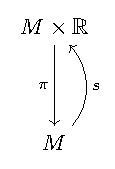
\includegraphics{lectures/7/pictures/cd_13.pdf}
 		 \end{center}

 		 где $M$~--- гладкое многообразие. Действительно, если $M$ покрыть атласом $\{ U_{\alpha} \}$, то $m \times \R$ покроется атласом $U_{\alpha} \times \R$. Тогда в каждой карте у нас будет происходить всё то же самое, что и в случае $\R^n \times \R$. Так как внешний дифференциал коммутирует с пуллбэком, это не будет зависеть от выбора координат и мы получим, что в каждой карте (а значит и на всём многообразии)  у нас вновь есть карты двух типов и мы можем совершенно аналогично построить цепную гомотопию $K$. Таким образом, получаем 

 		 \begin{corollary}
 		 	$H^{q}_{\dR}(M \times \R) \cong H^{q}(M)$. 
 		 \end{corollary}

 		 Отсюда мы получаем гомотопиечскую инвариантность когомологий де-Рама:

 		 \begin{corollary}
 		  	Гомотопные гладкие отображения индуцируют одинакоые отоюражения в когомологиях.
 		  \end{corollary} 
 		  \begin{remark}
 		  	Пусть $f, g \colon M \to N$. Под гладкой гомотопией мы тут понимаем такое отображение $H\colon M \times \R \to N$, что 
 		  	\[
 		  		H(x, t) = \begin{cases} f(x), & t \ge 1 \\ g(x), & t \le 0. \end{cases}
 		  	\]
 		  \end{remark}
 		  \begin{proof}
 		  		Пусть $H$~--- гомотопия между $f$ и $g$. Тогда у нас есть такая диаграмма: 

 		  		\begin{center}
 		  			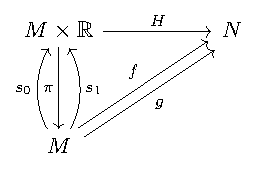
\includegraphics{lectures/7/pictures/cd_14.pdf}
 		  		\end{center}
 		  		то есть $f = H \circ s_1, \ g = H \circ s_0$. Тогда $f^* = s_1^* \circ H^*$, $g^* = s_0^* \circ H^*$, а тогда, так как $s_1^*$ и $s_0^*$ оба обратные к $\pi^*$, отсюда ясно, что $f^* = g^*$. 
 		  \end{proof}

 		  \begin{corollary}
 		  	Гомотопически эквивалентные многообразия имеют однаковые когомологии де Рама. 
 		  \end{corollary}

 		  Действительно, тут нужно просто воспользоваться функториальностью когомологий. 

 		  \begin{remark}
 		  		При всех разговорах про гомотопии, мы подразумеваем, что читателю известно, что любое непрерывное отображение гомотопно гладкому, и в частнсоти, что гомотопию тоже можно всегда выбирать гладкой (так как отображения можно сглаживать с фиксацией на подмножестве). 
 		  \end{remark}

 		  \begin{corollary}
 		  	В частности, деформационная ретракция индуцирует тождественное отображение в когомологиях. 
 		  \end{corollary}

 		  \subsection{Когомологии сферы}

 		  Покроем $S^n$ двумя дисками $U$ и $V$ так, чтоб верхнее немножко наезжало на нижнее и применим точную послеовательность Майера-Виеториса. Перед этим отметим, что $U \cap V \cong S^{n - 1} \times \R$. Тогда 
 		  \begin{center}
 		  		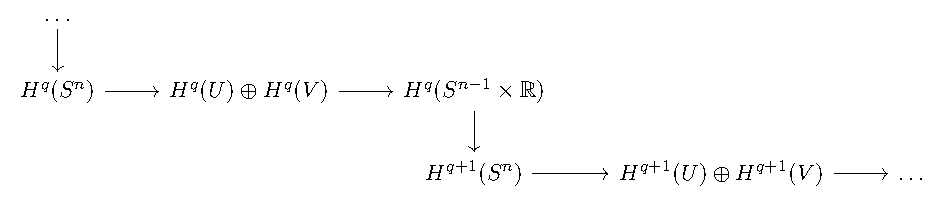
\includegraphics{lectures/7/pictures/cd_15.pdf}
 		  \end{center}

 		  Так как диск диффеоморфен $\R^n$, по лемме Пуанкаре $H^{q}_{\dR}(U) = H^{q}_{\dR}(V) = 0$ при $q \neq 0$. Кроме того, по следствию леммы Пуанкаре $H^{q}(S^{n - 1} \times \R) = H^q(S^{n - 1})$, то есть на самом деле последовательность выглядит вот так: 

 		  \begin{center}
 		  	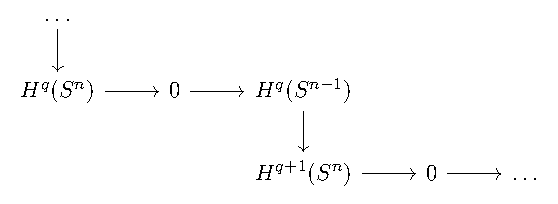
\includegraphics{lectures/7/pictures/cd_16.pdf}
 		  \end{center} 

 		  Отсюда мы сразу имеем 
 		  \[
 		  	 H^{q + 1}(S^{n}) \cong H^{q}(S^{n - 1}),
 		  \]
 		  откуда по индукции мы сразу получаем 
 		  \[
 		  	H^{q}(S^n) = \begin{cases} \R, & q = n \text{ или } 0. \\ 0, & q \neq n. \end{cases}
 		  \]

 		  Точнее говоря, случай $q = 0$ нужно разобрать отдельно руками. 

 		  \noindent\bf{Форма объема для сферы}

 		  Пусь $\sum x_i^2 = r^2$, тогда форма 
 		  \[
 		  	\omega = \frac{1}{r} \sum_{j = 1}^{n} x_j \mathrm{d}x_1 \wedge \ldots \wedge \overline{ \mathrm{d}x_j} \wedge \mathrm{d}x_n
 		  \]
 		  будет формой объема для сферы, то есть
 		  \[
 		  	\int\limits_{S^{n - 1}} \omega = \Vol_{n - 1}(S^{n - 1}).
 		  \]
 		  Заметим, что $\mathrm{d}\omega \in H^{n}(S^{n - 1})$, а значит, $[\mathrm{d}\omega] = 0$ просто из соображений размерности. С другой же стороны, эта форма не может быть точной, так как если $\omega = \mathrm{d}\alpha$, то тогда по формуле Стокса 

 		  \[
 		  	\int\limits_{S^{n - 1}} \omega = \int\limits_{B_{1}} \mathrm{d}\omega = \int\limits_{B} d^2 \alpha = 0.
 		  \]

 		  Значит, мы явно нашли образующую $H^n_{\dR}(S^n)$.



 		  \subsection{Лемма Пуанкаре для компактных когомологий}

 		  Мы будем доказывать, что 
 		  \[
 		  	H^{q + 1}_{c}(\R^n \times \R) = H^{q}_{c}(\R^n).
 		  \]
 		  \begin{remark}
 		  	Рассмотрим сначала общую ситуацию: пусть $\pi\colon M \times \R \to M $~--- проекция. Тогда пулбек формы из $\Omega_{c}^{\bullet}(M)$ уже не имеет компактного носителя (так как она постоянна вдоль слоёв). 

 		  	Однако, есть отображение интегрирования вдоль слоя: 
 		  	\[
 		  		\pi_*\colon \Omega_{c}^{\bullet}(M \times \R) \to \Omega_{c}^{\bullet - 1}(M)).
 		  	\]
 		  	Оно определяется по отдельности на формах двух типов: 
 		  	\begin{itemize}
 		  		\item $\pi_*(\varphi f(x, t)) = 0$.
 		  		\item $\pi_*(\varphi f(x, t) \mathrm{d}t) = \varphi \int\limits_{-\infty}^{+\infty} f(x, t) \mathrm{d}t$.

 		  		Интеграл тут определён корректно, так как форма имела компактный носитель. 
 		  	\end{itemize}
 		  \end{remark}

 		  Нетрудно проверить, что $\mathrm{d} \pi_* = \pi_* \mathrm{d}$. Определим также отображение 
 		  \[
 		  	e_*\colon \Omega_c^{\bullet}(M) \to \Omega^{\bullet + 1}_{c}(M \times \R), \ \varphi \mapsto (\pi^* \varphi) \wedge e, 
 		  \]
 		  где $e$~--- это форма с компактным носителем на $\R$ такая, что $\int_{\R} e = 1$. 

 		  Очевидно, что $\pi_* \circ e_* = \id$ на $\Omega_{c}^{\bullet}(\R^n)$. А вот $e_* \circ \pi_*$ уже не тождественно на уровне форм, но, опять же, цепногомотопно тождественному отображению. Это проверяется также, как и для обычных когомологий де Рама. 

 		  Отсюда мы получаем, что 
 		  \[
 		  	H_c^{q}(\R^n) = \begin{cases} \R, & q = n \\ 0, & \text{ иначе }\end{cases}. 
 		  \]

 		  Причём, изоморфизм тут такой же, как был у нас в случае $\R^1$: 
 		  \[
 		  	\omega \mapsto \int\limits_{\R^n} \omega 
 		  \]

 		  Образующей $H^n_{c}(\R^n)$ будет форма 
 		  \[
 		  	e(x_1) \mathrm{d}x_1 \wedge e(x_2) \mathrm{d}x_2 \wedge \ldots \wedge e(x_n) \mathrm{d}x_n. 
 		  \]

 		  \begin{remark}
 		  	Отсюда также можно уследить, что когомологии с компактным носителем не гомотопически инвариантны. Чтоб в этом убедиться, можно, например, вычислить компактные когомологии открытого цилиндра и открытого листа Мёбиуса. 
 		  \end{remark}

 		  

 		  \subsection{Умножение в когомологиях де Рама}

 		  Вообще говоря, при помощи $\wedge$-произведения можно умножать формы, что наводит на мысль о том, что это может превращать когомологии в градуированное кольцо. Покажем, что это действительно так, то есть, что умножение 
 		  \[
 		  	\wedge\colon \Omega^k(M) \times \Omega^{\ell}(M) \to \Omega^{k + \ell}(M), \quad (w, v) \mapsto w \wedge v
 		  \]
 		  продолжается до умножения в когомологиях. Определим умножение в когомологиях следующим образом: 
 		  \[
 		  	\wedge \colon H^k(M) \times H^{\ell}(M) \to H^{k + \ell}(M), \quad [w] \wedge [v] = [w \wedge v]. 
 		  \]
 		  Покажем, что это определение корректно, т.е. не зависит от выборов представителей. Нам надо показать, что 
 		  \[
 		  	[(w + \mathrm{d}\alpha) \wedge (v + \mathrm{d}\beta)] = [w \wedge v]
 		  \]
 		  для замкнутых форм $w \in \Omega^k(M), \ v \in \Omega^{\ell}(M)$ и произвольных $\alpha \in \Omega^{k - 1}(M), \ \beta \in \Omega^{\ell - 1}(M)$. Действительно, 
 		  \[
 		  	(w + \mathrm{d}\alpha) \wedge (v + \mathrm{d}\beta) = w \wedge v + w \wedge \mathrm{d}\beta + \mathrm{d}\alpha \wedge v + \mathrm{d}\alpha \wedge \mathrm{d}\beta.
 		  \]
 		  Покажем, что всё кроме первого слагаемого~--- точная форма. Действительно, рассмотрим 
 		  \[
 		  	\tau = \alpha \wedge v + (-1)^{k} w \wedge \beta + \alpha \wedge \mathrm{d}\beta.
 		  \]
 		  Перед тем, как дифференцировать, напомним, что внешний дифференциал удовлетворяет правилу лейбница, то есть 
 		  \[
 		  	\mathrm{d}(w \wedge v) = \mathrm{d}w \wedge v + (-1)^k w \wedge \mathrm{d}v, \ w \in \Omega^k(M), \ v \in \Omega^{\ell}(M).
 		  \]
 		  Теперь продифференцируем форму $\tau$: 
 		  \[
 		  	\mathrm{d}\tau = \mathrm{d}\alpha \wedge v + (-1)^{k - 1}\alpha \wedge \mathrm{d}v + (-1)^k \mathrm{d}w \wedge \beta + w \wedge \mathrm{d}\beta + \mathrm{d}\alpha \wedge \mathrm{d}\beta.
 		  \]
 		  Теперь воспользуемся тем, что $\mathrm{d}w = \mathrm{d}v = 0$, тогда 
 		  \[
 		  	  \mathrm{d}\tau = \mathrm{d}\alpha \wedge v + w \wedge \mathrm{d}\beta + \mathrm{d}\alpha + \mathrm{d}\beta.
 		  \]
 		  Таким образом,  
 		  \[
 		  		(w + \mathrm{d}\alpha) \wedge (v + \mathrm{d}\beta) = w \wedge v + \mathrm{d}\tau \implies [(w + \mathrm{d}\alpha) \wedge (v + \mathrm{d}\beta)] = [w \wedge v]. 
 		  \]

 		  
 		  Таким образом, внешнее произведение превращает 
 		  \[
 		  	H^{\bullet}(M) = \bigoplus_{i = 1}^{\infty} H^{i}(M)
 		  \]
 		  в градуированное кольцо. 

        Теперь пусть у нас есть отображения $f$ и $g$, которые осуществляют гомотопическую эквивалентность многообразий $M$ и $N$. Заметим, что тогда просто по определению пуллбека, мы имеем 
        \[ 
            f^{*}(w \wedge v) = f^*(w) \wedge f^*(v) \quad \forall w \Omega^k(N), \ v \in \Omega^{\ell}(N).
        \]
        Так как при гомотопической эквивалентности $f^*$ и $g^*$~--- изоморфизмы на когомологиях, мы получаем, что $f^*$~--- изоморфизм градуированных алгебр $H^{\bullet}(N)$ и $H^{\bullet}(M)$.
    